\documentclass[a4paper]{report}
\usepackage{Rnews}
\usepackage[round]{natbib}
\usepackage{array}
\usepackage{graphicx}
\bibliographystyle{abbrvnat}

\begin{document}

\begin{article}
\author{by Nitin Jain and Gregory R. Warnes}
\title{Balloon Plot}
\subtitle{Graphical tool for displaying tabular data}

\maketitle

\section*{Introduction}

Numeric data is often summarized using rectangular tables. While
these tables allow presentation of all of the relevant data, they do
not lend themselves to rapid discovery of important patterns. The
primary difficulty is that the visual impact of numeric values is
not proportional to the scale of the numbers represented.

We have developed a new graphical tool, the \code{balloonplot},
which augments the numeric values in tables with colored circles
with area proportional to the size of the corresponding table
entry. This visually highlights the prominent features of
data, while preserving the details conveyed by the numeric values
themselves.

In this article, we describe the balloonplot, as
implemented by the \code{balloonplot} function in the
\code{gplots} package, and describe the features of our
implementation.


\section*{Function description}

The \code{balloonplot} function accepts a table (to be displayed as
found) or lists of vectors for x (column category), y (row category)
and z (data value) from which a table will be constructed.

The \code{balloonplot} function plots a graphical table,
where each cell displays the appropriate numeric value plus a
colored circle whose size reflects the relative magnitude of the
corresponding component. The
\emph{area} of each circle is proportional to the frequency of
data. (The circles are scaled so that the circle for largest value
fills the available space in the cell.)


As a consequence, the largest values in the table are ``spotlighted''
by the biggest circles, while the smaller values are displayed
with very small circles.  Of course, circles can only have positive
radius, so the radius of circles for cells with negative values are
set to zero.  (A warning is issued when this ``truncation'' occurs.)

Of course, when labels are present on the table or provided to the
function, the graphical table is appropriately labeled.  In
addition, options are provided to allow control of various visual features
of the plot:

\begin{itemize}
  \item rotation of the row and column headers
  \item balloon color and shape (globally or individually)
  \item number of displayed digits
  \item display of entries with zero values
  \item display of marginal totals
  \item display of cumulative histograms
  \item x- and y-axes group sorting
  \item formatting of row and column labels
  \item as well as the traditional graphics parameters (title,
    background, etc.)
\end{itemize}

\section*{Example using the \code{Titanic} data set}

For illustration purposes, we use the \code{Titanic} data set from
the \code{datasets} package.  \code{Titanic} provides survival status
for passengers on the tragic maiden voyage of the ocean liner
``Titanic'', summarized according to economic status (class), sex, and
age.

Typically, the number of surviving passengers are shown in a tabular
form, such as shown in Figure~\ref{figure:Figure1}.  (This was created
by calling balloonplot with the balloon color set to match the
background color and most options disabled.)  Note that one must
actively focus on the individual cell values in order to see any
pattern in the data.

\begin{figure}
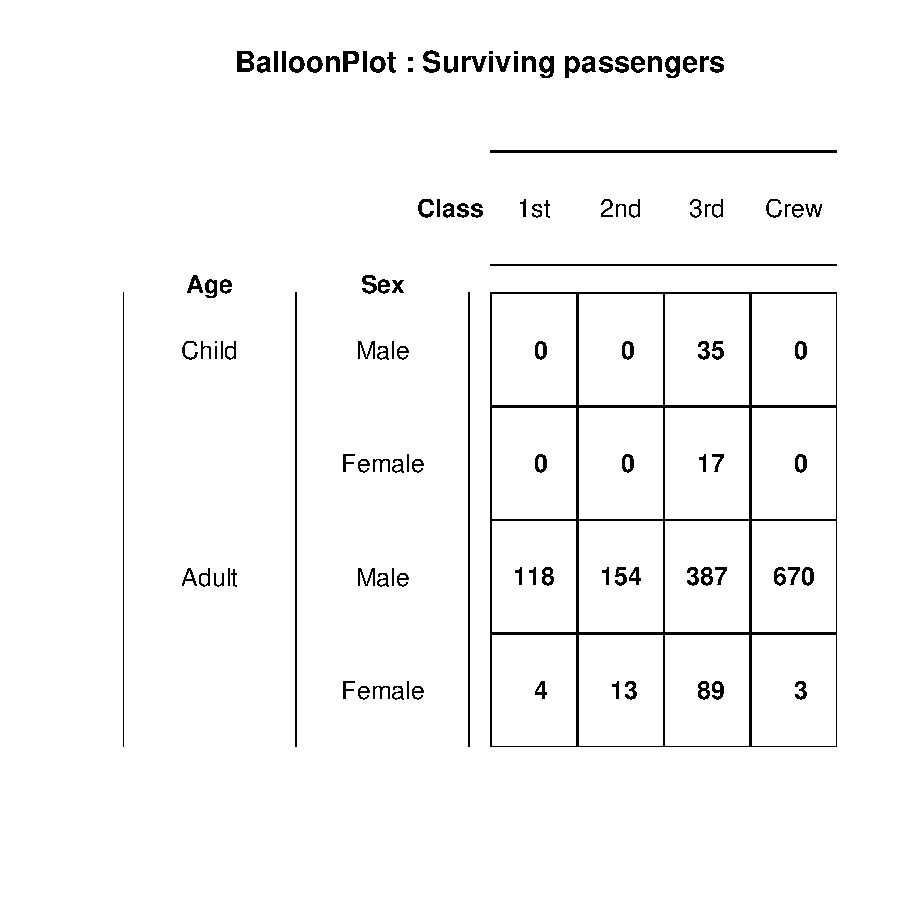
\includegraphics[width=\textwidth]{Figure1.pdf}
\caption{\label{figure:Figure1}
Tabular representation of survived population by gender and age}
\end{figure}


Now, we redraw the table with light-blue circles (`balloons')
superimposed over the numerical values (figure~\ref{figure:Figure2}).
This is accomplished using the code:

{\small
\begin{verbatim}
data(Titanic)

# Convert to 1 entry per row format
dframe <- as.data.frame(Titanic) 

# Select only surviving passengers
survived <- dframe[dframe$Survived=="Yes",]
attach(survived)

balloonplot(x=Class,
            y=list(Age, Sex),
            z=Freq,
            sort=TRUE,
            show.zeros=TRUE,
            dotcol=''green'',
            cum.margins=FALSE,
            main=
            "BalloonPlot : Surviving passengers"
            )

title(main=list("Circle area is proportional to\
 number of passengers",
           cex=0.9),
      line=0.5)

detach(survived)
\end{verbatim}
}
%$

\begin{figure}
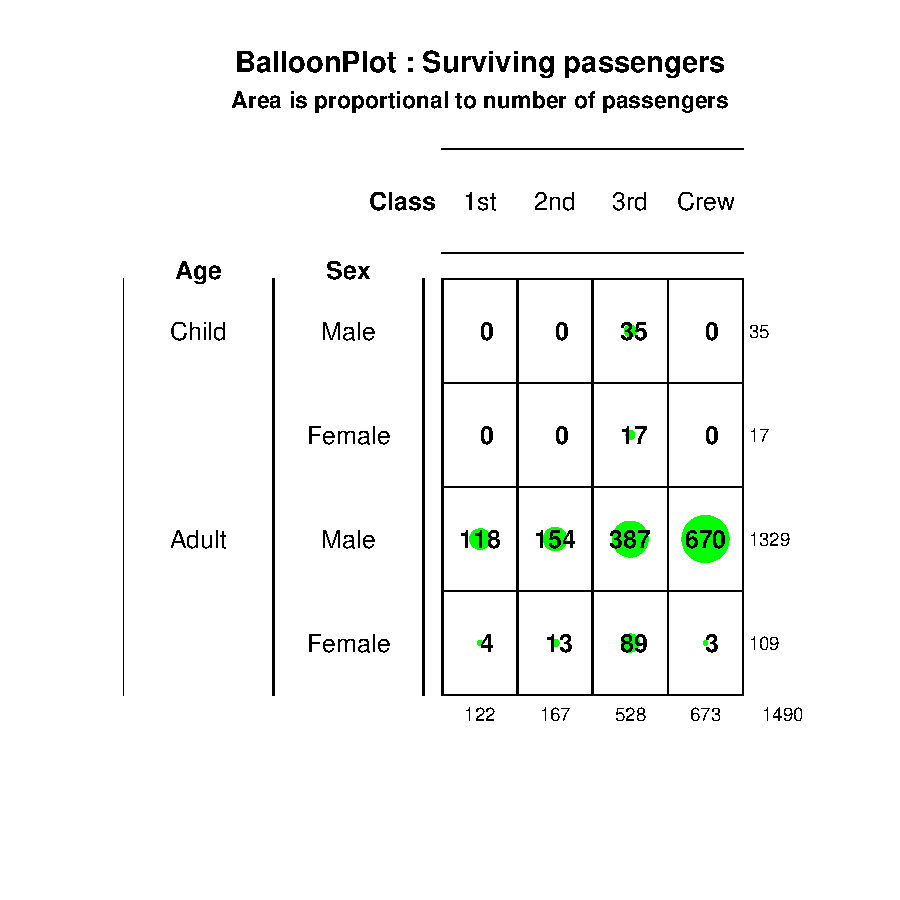
\includegraphics[width=\textwidth]{Figure2.pdf}
\caption{\label{figure:Figure2}
Balloon plot of surviving individuals by class, gender and age }
\end{figure}

With the addition of the blue ``spotlights'', whose area is
proportional to the magnitude of the data value, it is easy to see
that only adult females and adult male crew members survived in
large numbers.  Note the addition of row and column marginal
totals.

Of course, the number of surviving passengers is only half of the
story.  We could create a similar plot showing the number of
passengers who did not survive.  Alternatively, we can simply add
survival status as another variable to the display, setting the color
of the circles to green for passengers who survived, and magenta for
those who did not:

\begin{figure}
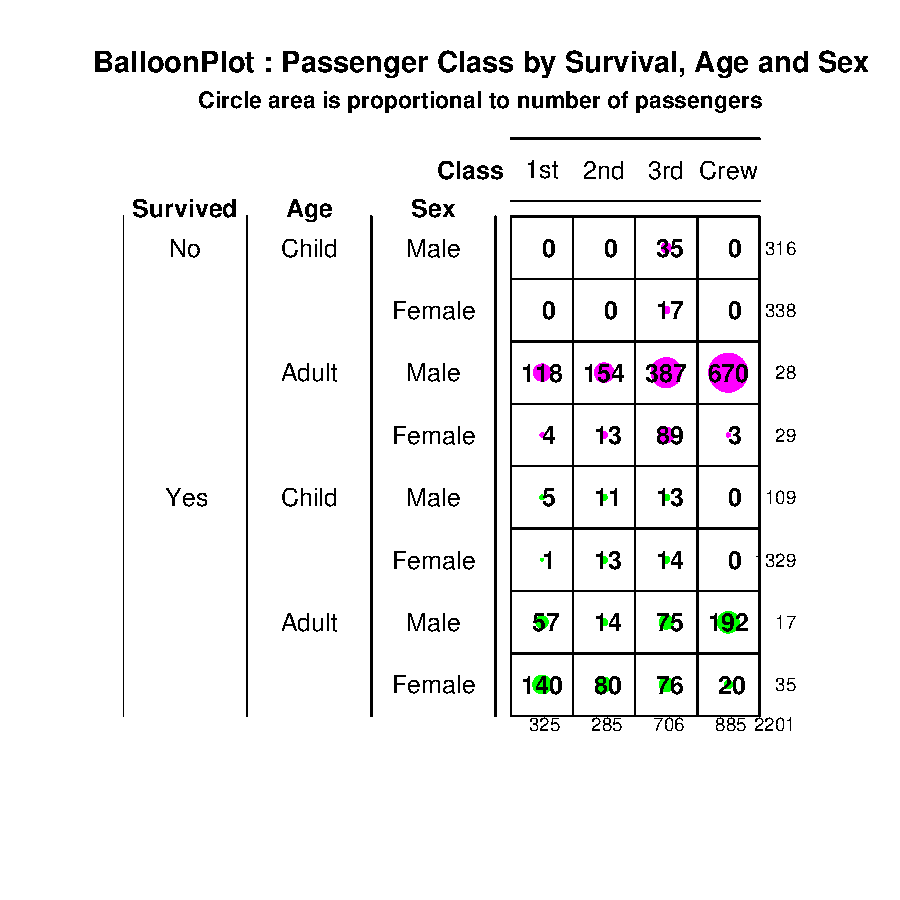
\includegraphics[width=\textwidth]{Figure3.pdf}
\caption{\label{figure:Figure3}
  Balloon plot of Titanic passengers by gender, age and class. Green
  circles represent passengers who survived and magenta circles
  represent the passengers who did not survive.}
\end{figure}

Figure~\ref{figure:Figure3} conveys considerably more information than
figures 1 and 2 without substantial loss of clarity. The large magenta
circles make it clear that most passengers did not survive.

To further improve the display, we add a visual representation of
the row and column sums using grey bars behind the row and column
headers (figure 4).  This is accomplished using the code:

{
\small
\begin{verbatim}
attach(dframe)
colors <- ifelse( Survived=="Yes", "green", 
                  "magenta")

balloonplot(x=Class,
            y=list(Survived, Age, Sex),
            z=Freq,
            sort=FALSE,
            dotcol=colors,
            show.zeros=TRUE,
            main="BalloonPlot : Passenger Class \
by Survival, Age and Sex"
            )

points( x=1, y=8, pch=20, col="magenta")
points( x=1, y=4, pch=20, col="green")

title(main=list("Circle area is proportional to \
number of passengers",
           cex=0.9),
      line=0.5)

detach(dframe)
\end{verbatim}
 }
%$

\begin{figure}
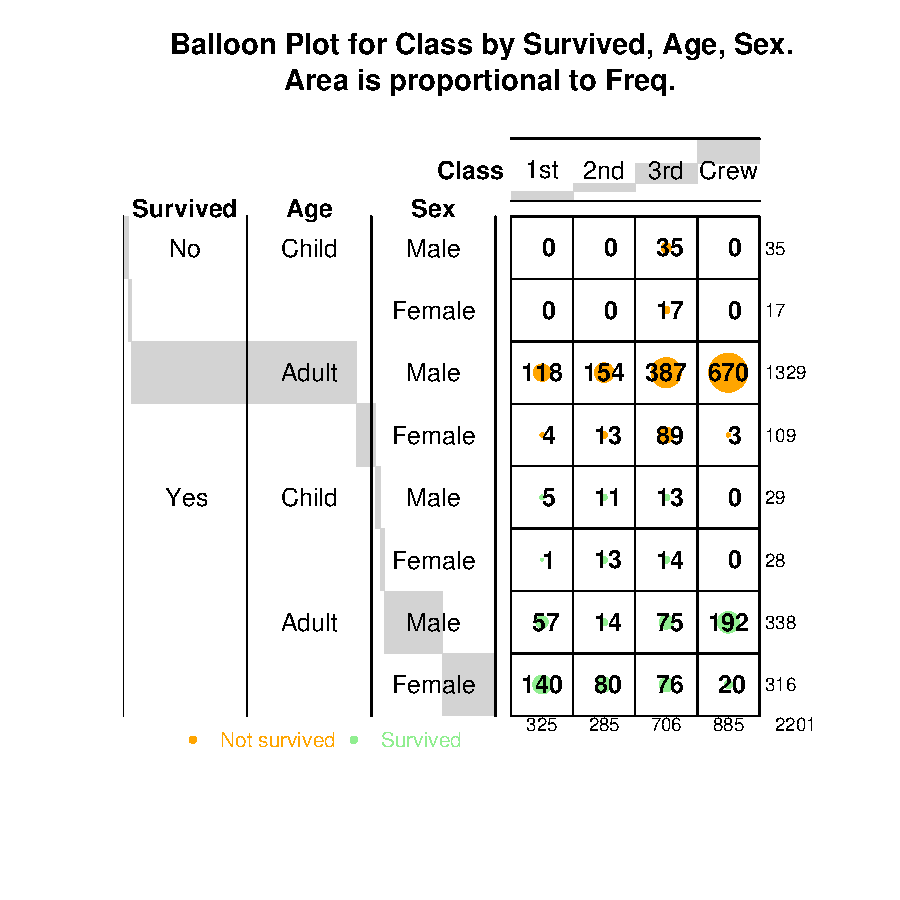
\includegraphics[width=\textwidth]{Figure4.pdf}
\caption{\label{figure:Figure4}
Balloon plot of all the passengers of Titanic, stratified by survival,
age, sex and class}
\end{figure}

It is now easy to see several facts:
\begin{itemize}
\item A surprisingly large fraction (885/2201) of passengers were crew
      members
\item Most passengers and crew were adult males 
\item Most adult males perished
\item Most women survived, except in $3^{rd}$ class
\item Only 3rd class children perished
\end{itemize}

Perhaps the most striking fact is that survival is lowest among
$3^{rd}$ class passengers for all age/gender groups.  It turns out
that there is a well known reason for this difference in survival.
Passengers in $1^{st}$ and $2^{nd}$ class, as well as crew members,
had better access to the lifeboats.  Since there were too few
lifeboats for the number of passengers and crew, most women and
children among the $1^{st}$ class, $2^{nd}$ class and crew found space
in a lifeboat, while many of the later arriving $3^{rd}$ class women
and children were too late: the lifeboats had already been filled and
had moved away from the quickly sinking ship.

\section*{Conclusion}

Using the well worn Titanic data, we have shown how balloonplots
help to convey important aspects of tabular data, without obscuring
the exact numeric values. We hope that this new approach to
visualizing tabular data will assist other statisticians in more
effectively understanding and presenting tabular data.

We wish to thank \emph{Ramon Alonso-Allende}
\email{allende@cnb.uam.es} for the discussion on R-help which lead
to the development of \code{balloonplot}, as well as for the code for
displaying the row and column sums.

\address{Gregory R. Warnes, Pfizer Inc., USA\\
\email{gregory.r.warnes@pfizer.com}\\
       Nitin Jain, The Cambridge Group, LTD., USA\\
\email{nitin.jain@pfizer.com}}

\end{article}

\end{document}
